%! TEX root = ../main.tex
\documentclass[../main.tex]{subfiles}

\begin{document}

\subsection{Fenditura $\qty{0.08}{\milli\metre}$}

Per la fenditura da $\qty{0.08}{\mm}$ ed apertura del sensore pari a $\qty{1.5}{\mm}$ sono stati raccolti $3$ set di dati che sono riportati in \autoref{fig:single scatter 0.08}.

\begin{figure}[ht!]
    \centering
    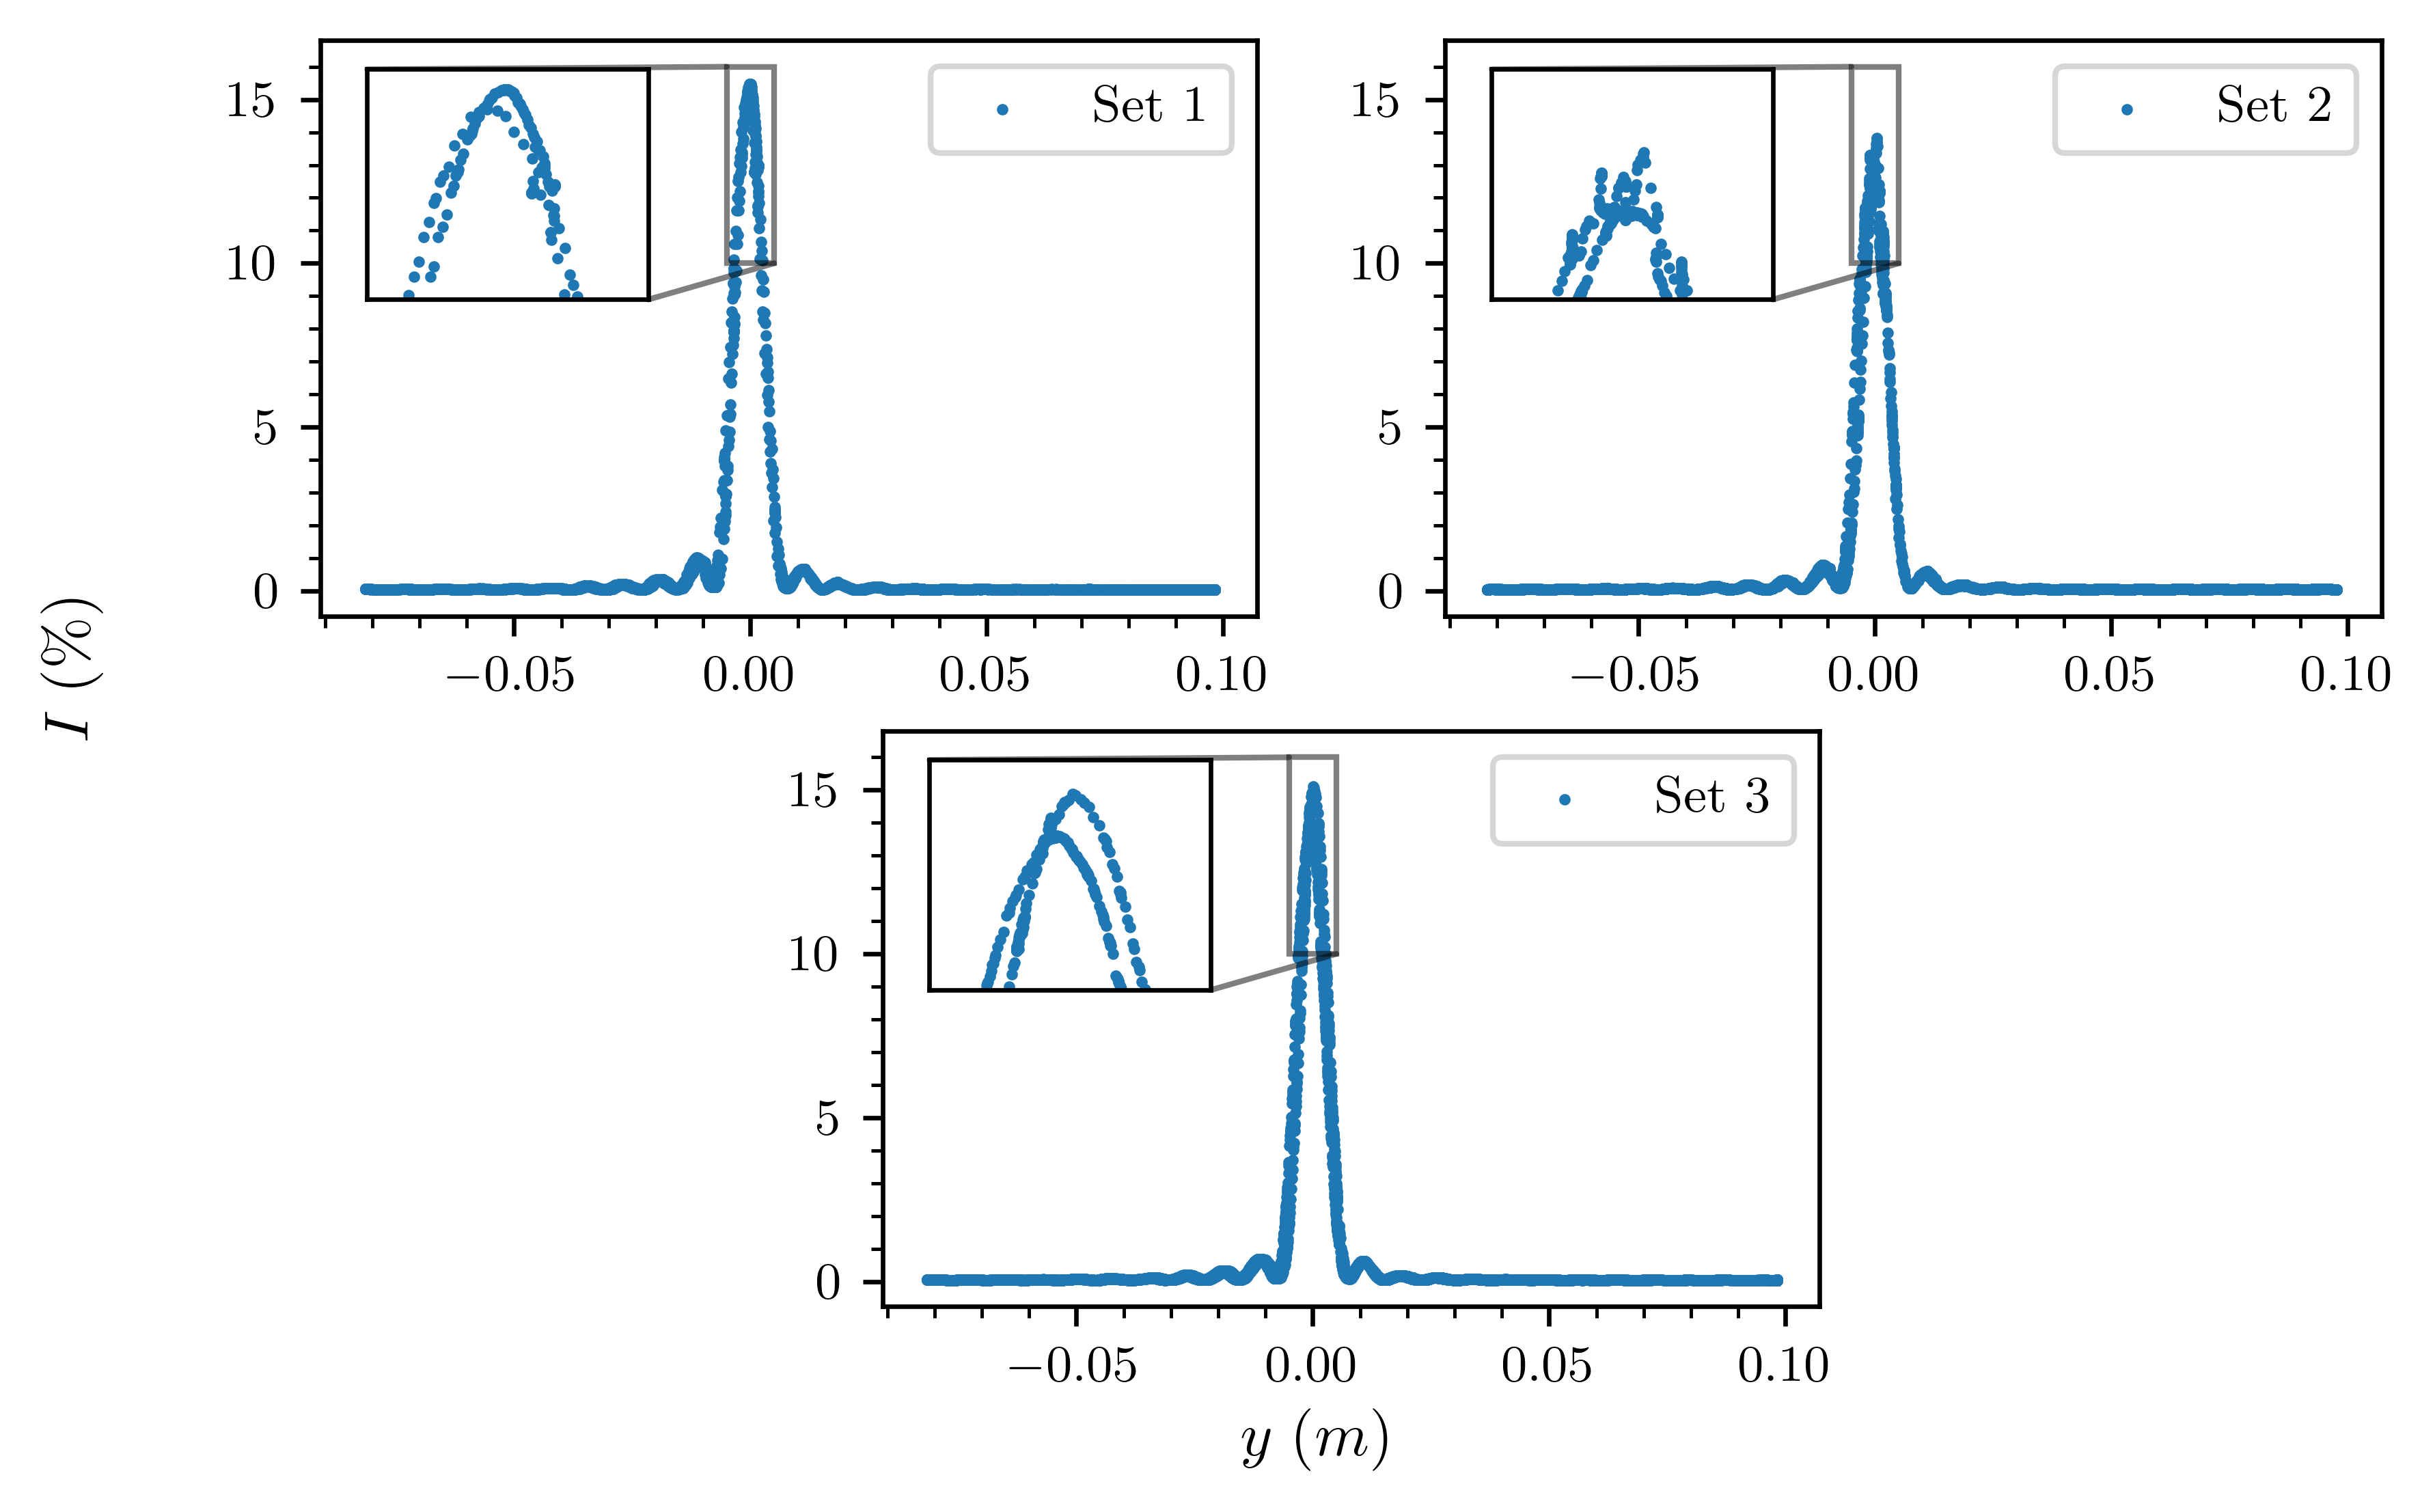
\includegraphics{single_scatter_0.08.png}
    \caption{Misure dell'intensità luminosa $I$ in funzione della posizione $y$ (in metri) del sensore.} %todo: aggiungere un commento
    \label{fig:single scatter 0.08}
\end{figure}

Sovrapponendo i set si è proceduto ad individuare la posizione dei minimi attribuendogli una barra d'errore sufficientemente grande da rendere la misura compatibile con tutti i set. Le posizioni dei minimi ottenute dalla \autoref{fig:minimi 0.08} sono riportate in \autoref{tab:minimi 0.08} di fianco ai valori della fenditura ricavati utilizzando l'\autoref{eq:y=0 values}.

\begin{figure}[ht!]
    \centering
    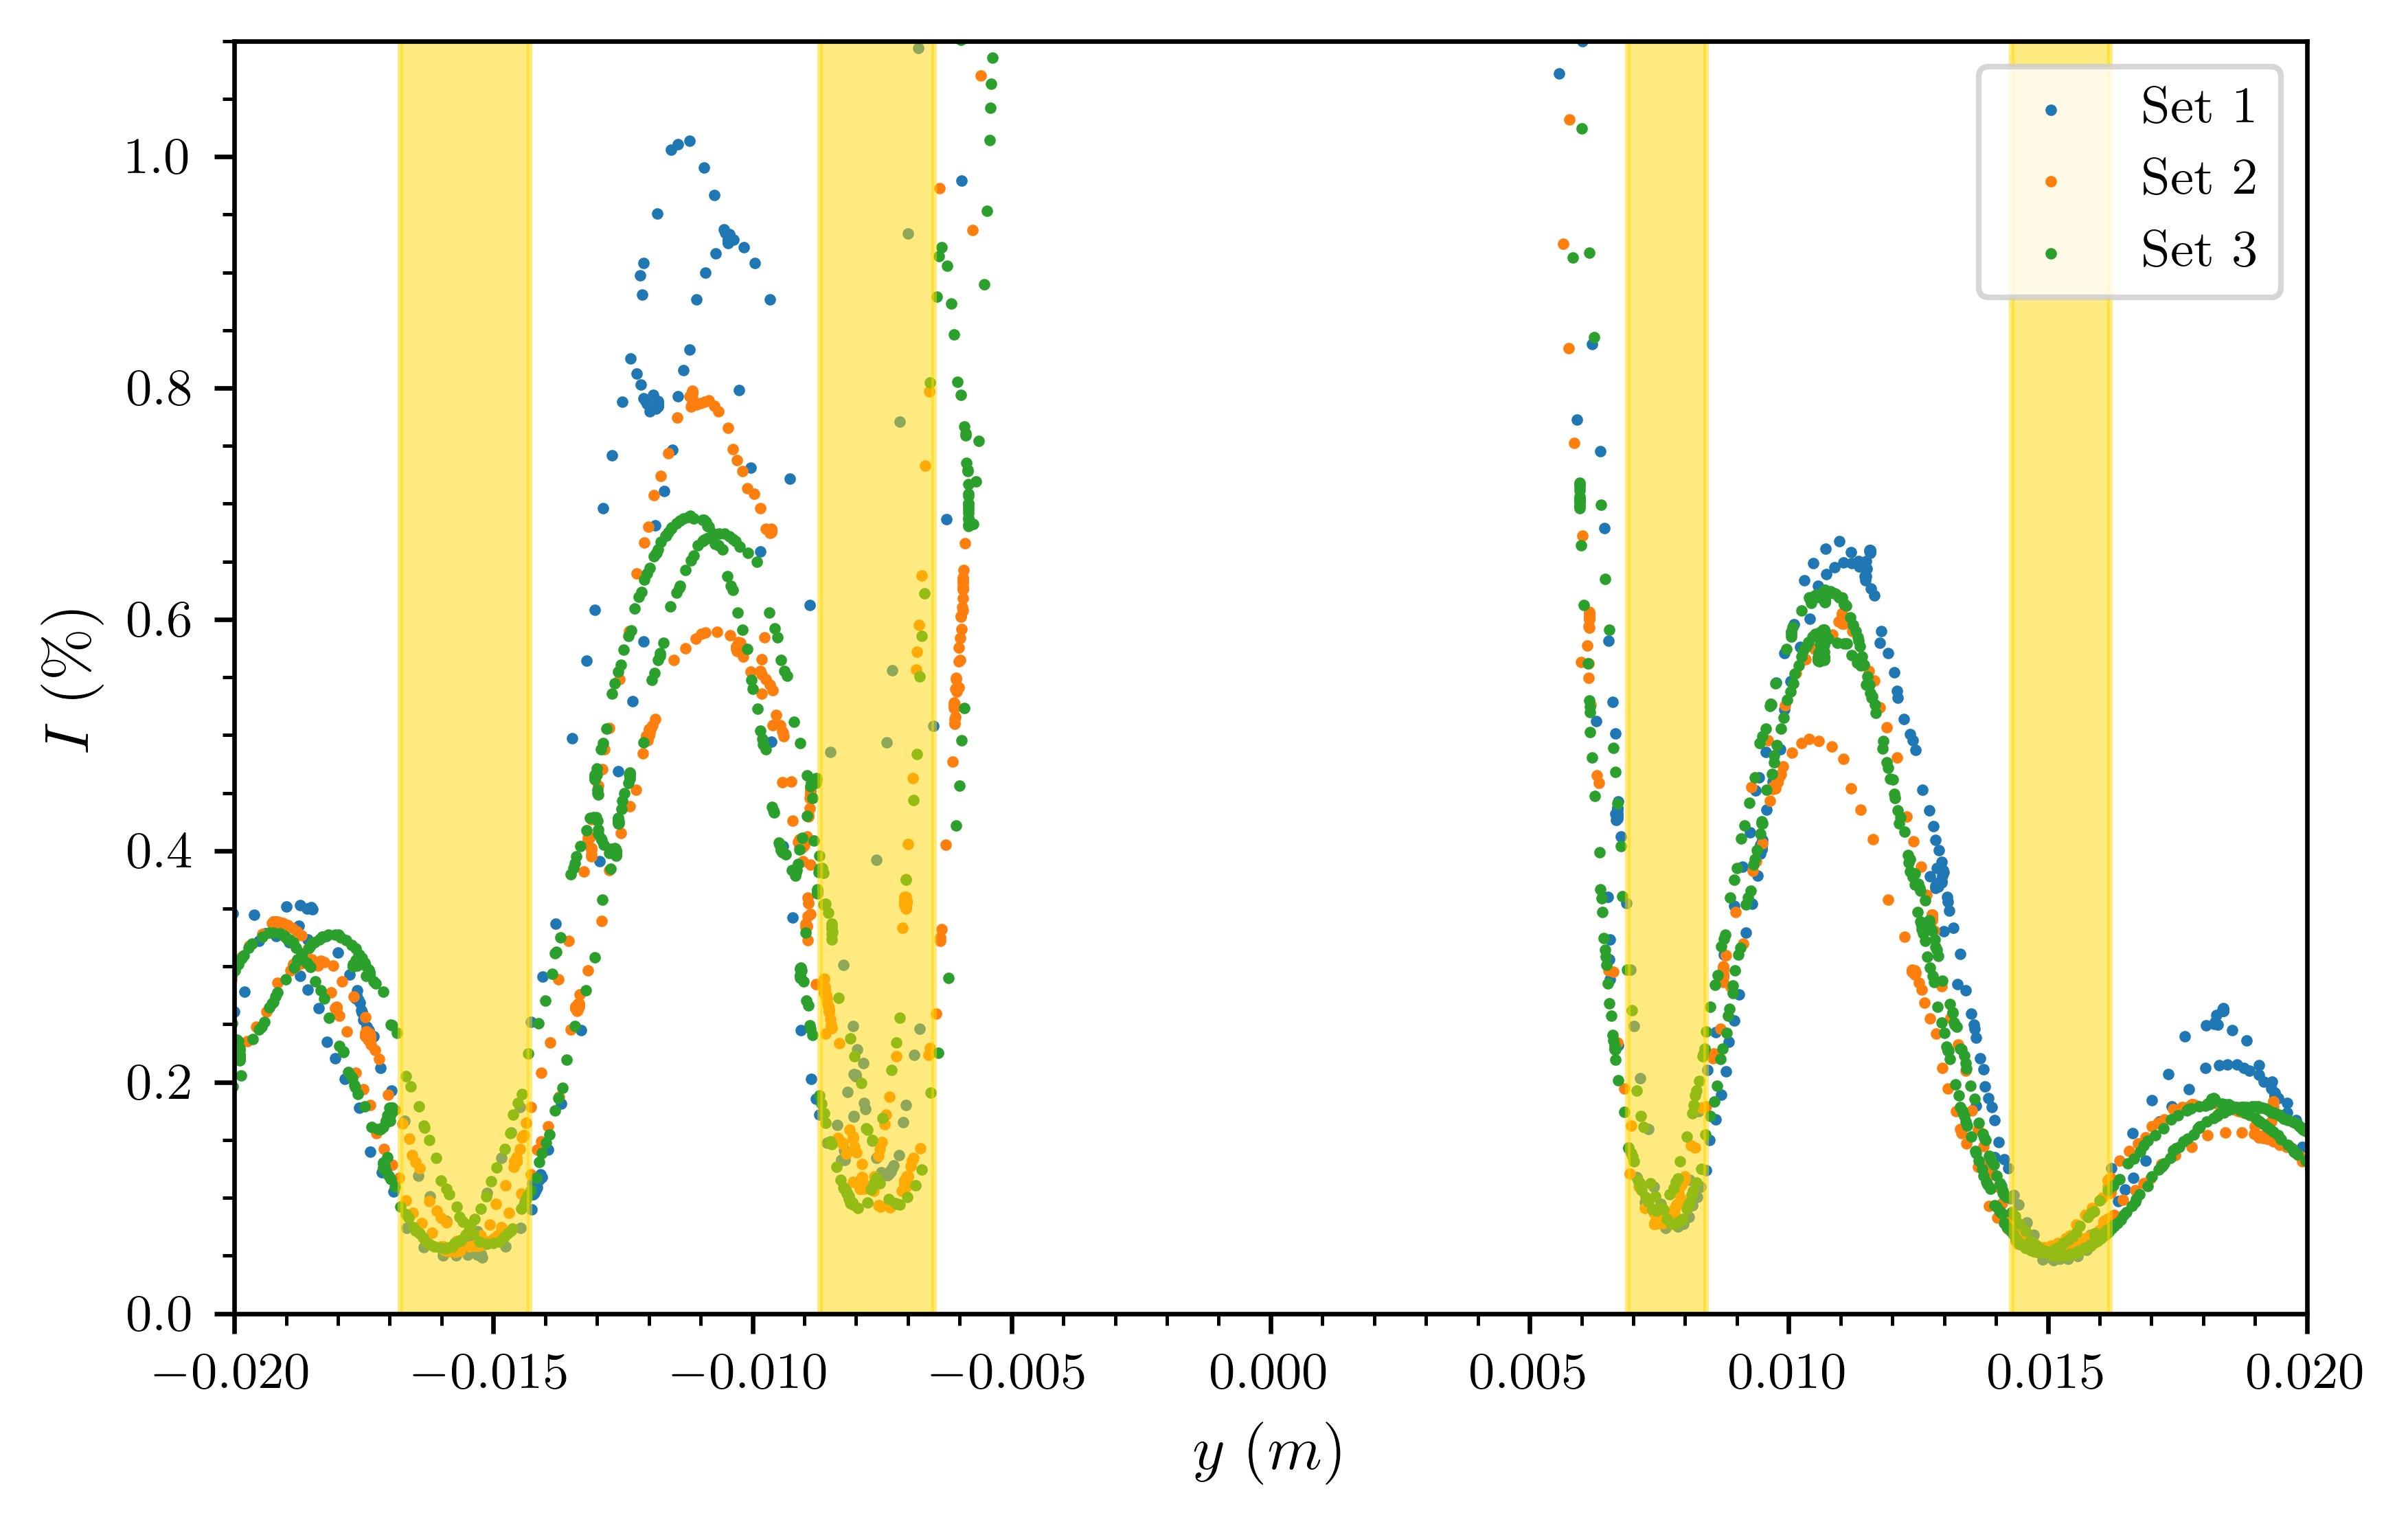
\includegraphics{min_0.08.png}
    \caption{Intensità luminosa $I$ in funzione della posizione $y$ del sensore (in metri) per la fenditura a $\qty{0.08}{\mm}$. Si può notare una forte asimmetria dei picchi laterali che risultano essere più bassi nella parte destra della curva.} %todo: aggiungere qualcosa in più alla descrizione
    \label{fig:minimi 0.08}
\end{figure}

\begin{table}[ht!]
    \centering
    \caption{Posizione dei minimi, ottenuta graficamente dalla \autoref{fig:minimi 0.08}, riportata di fianco al proprio indice $m$ ed al valore $a$ (in $\si{\mm}$) stimato seguendo la relazione esposta in \autoref{eq:y=0 values}. Il valore di $a$ derivato da ciascun minimo è stato ricavato ponendo $\lambda = \qty{650}{\nm}$ ed $L = \qty{98.5+-0.1}{\cm}$, per l'errore $\delta a$ sono stati sommati in quadratura i contributi di $\delta y$ e $\delta L$, così facendo il contributo di $\delta L$ risulta essere trascurabile.}
    \import{../tables/}{mins_0.08.tex}
    \label{tab:minimi 0.08}
\end{table}

Intersecando le barre d'errore dei valori ottenuti si ha $a_g = \qty{0.084+-0.005}{\mm}$ che risulta compatibile con il valore teorico.

\newpage

Successivamente si è proceduto con il fit utilizzando l'\autoref{eq:fit} e ottenendo un valore della fenditura $a_f = \qty{0.084+-0.007}{\mm}$, il grafico del fit è riportato in \autoref{fig:fit 0.08}.

\begin{figure}[ht!]
    \centering
    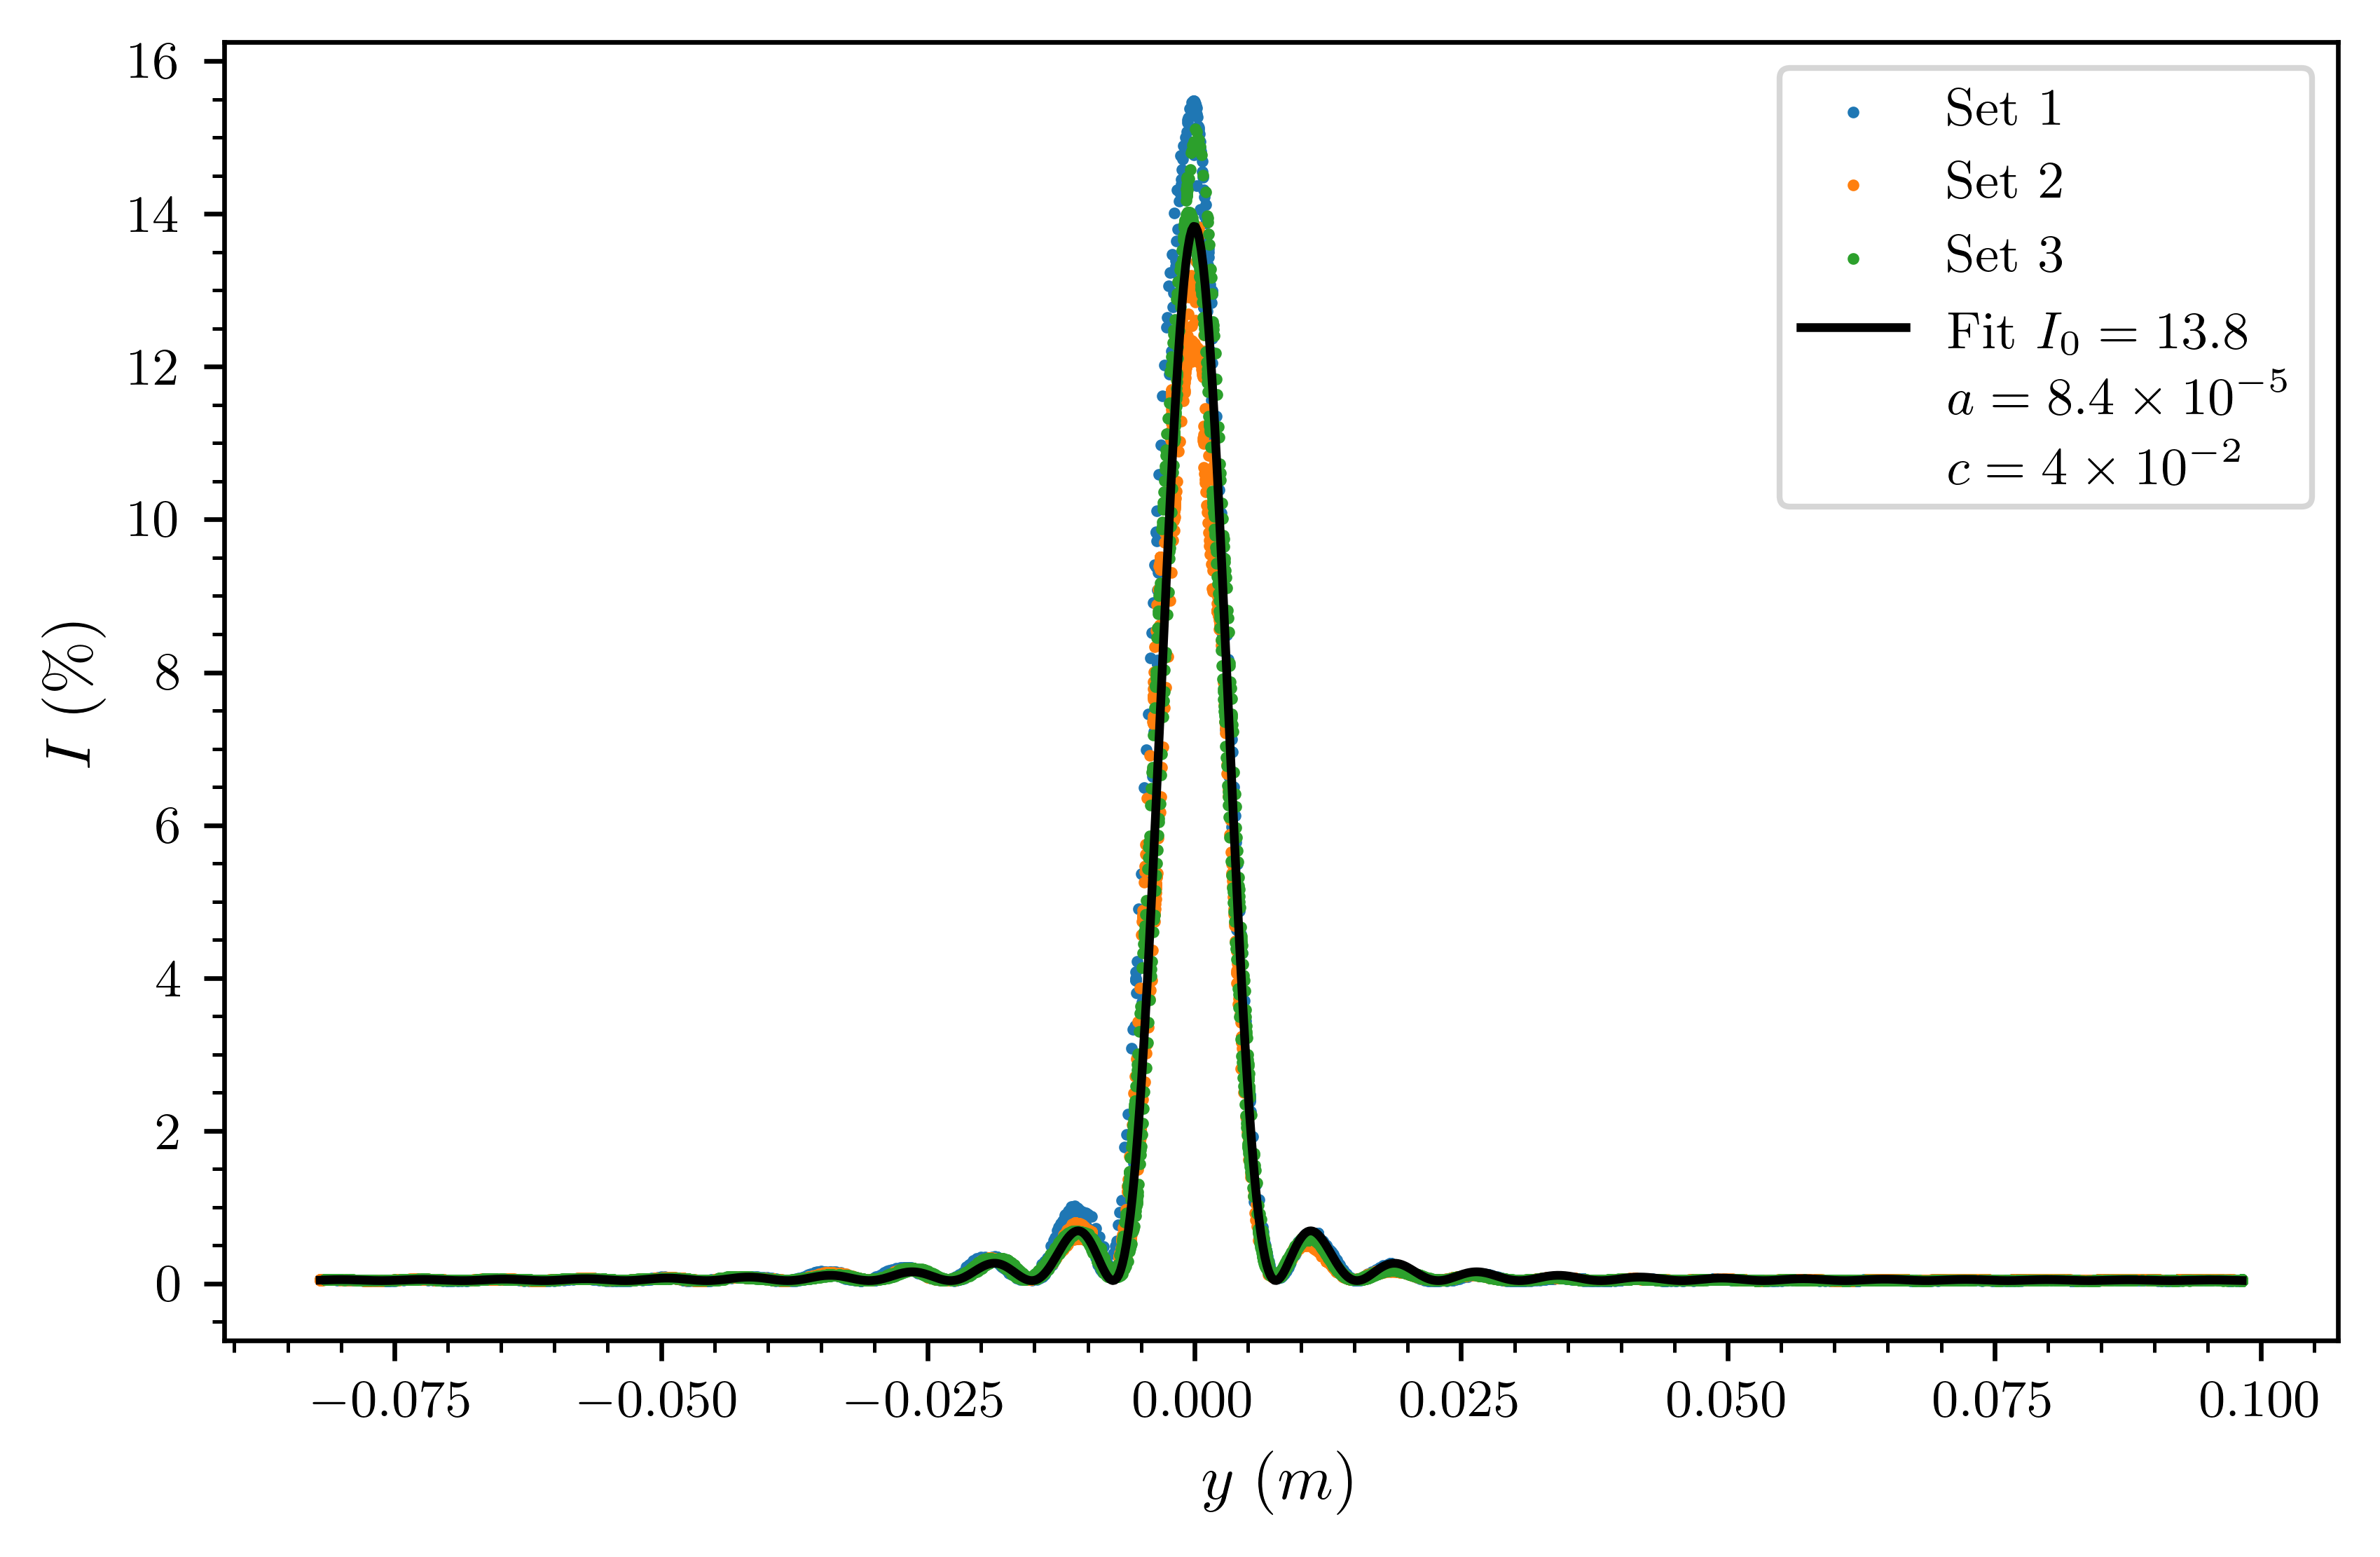
\includegraphics{fit_0.08.png}
    \caption{Intensità luminosa $I_{0}$ in funzione della posizione $y$ del sensore (in metri) per la fenditura a $\qty{0.08}{\mm}$. In figura è riportato il fit fatto utilizzando l'\autoref{eq:fit}. I valori dei parametri ottenuti sono $I_{0} = \num{13.8+-1.6}$, $a = \qty{0.084+-0.007}{\mm}$ e $c = \num{4+-1.2e-2}$.}
    \label{fig:fit 0.08}
\end{figure}

Entrambi $a_g$ e $a_f$ risultano compatibili con il valore teorico di $a = \qty{0.08}{\mm}$.

Per confrontare le misure ottenute con diverse aperture del sensore si è scelto di utilizzare il set $1$ delle misure con apertura $\qty{1.5}{\mm}$, in quanto presenta una variazione trascurabile dell'intensità massima. %? review: si può trovare un motivo migliore (tipo: il secondo set ha un picco orribile)
Dopo aver scalato le intensità dei set utilizzati in modo che il valore massimo di $I$ risultasse pari ad $1$ per tutti i set, essi sono stati riportati sovrapposti in \autoref{fig:sensore 0.08}.

\begin{figure}[ht!]
    \centering
    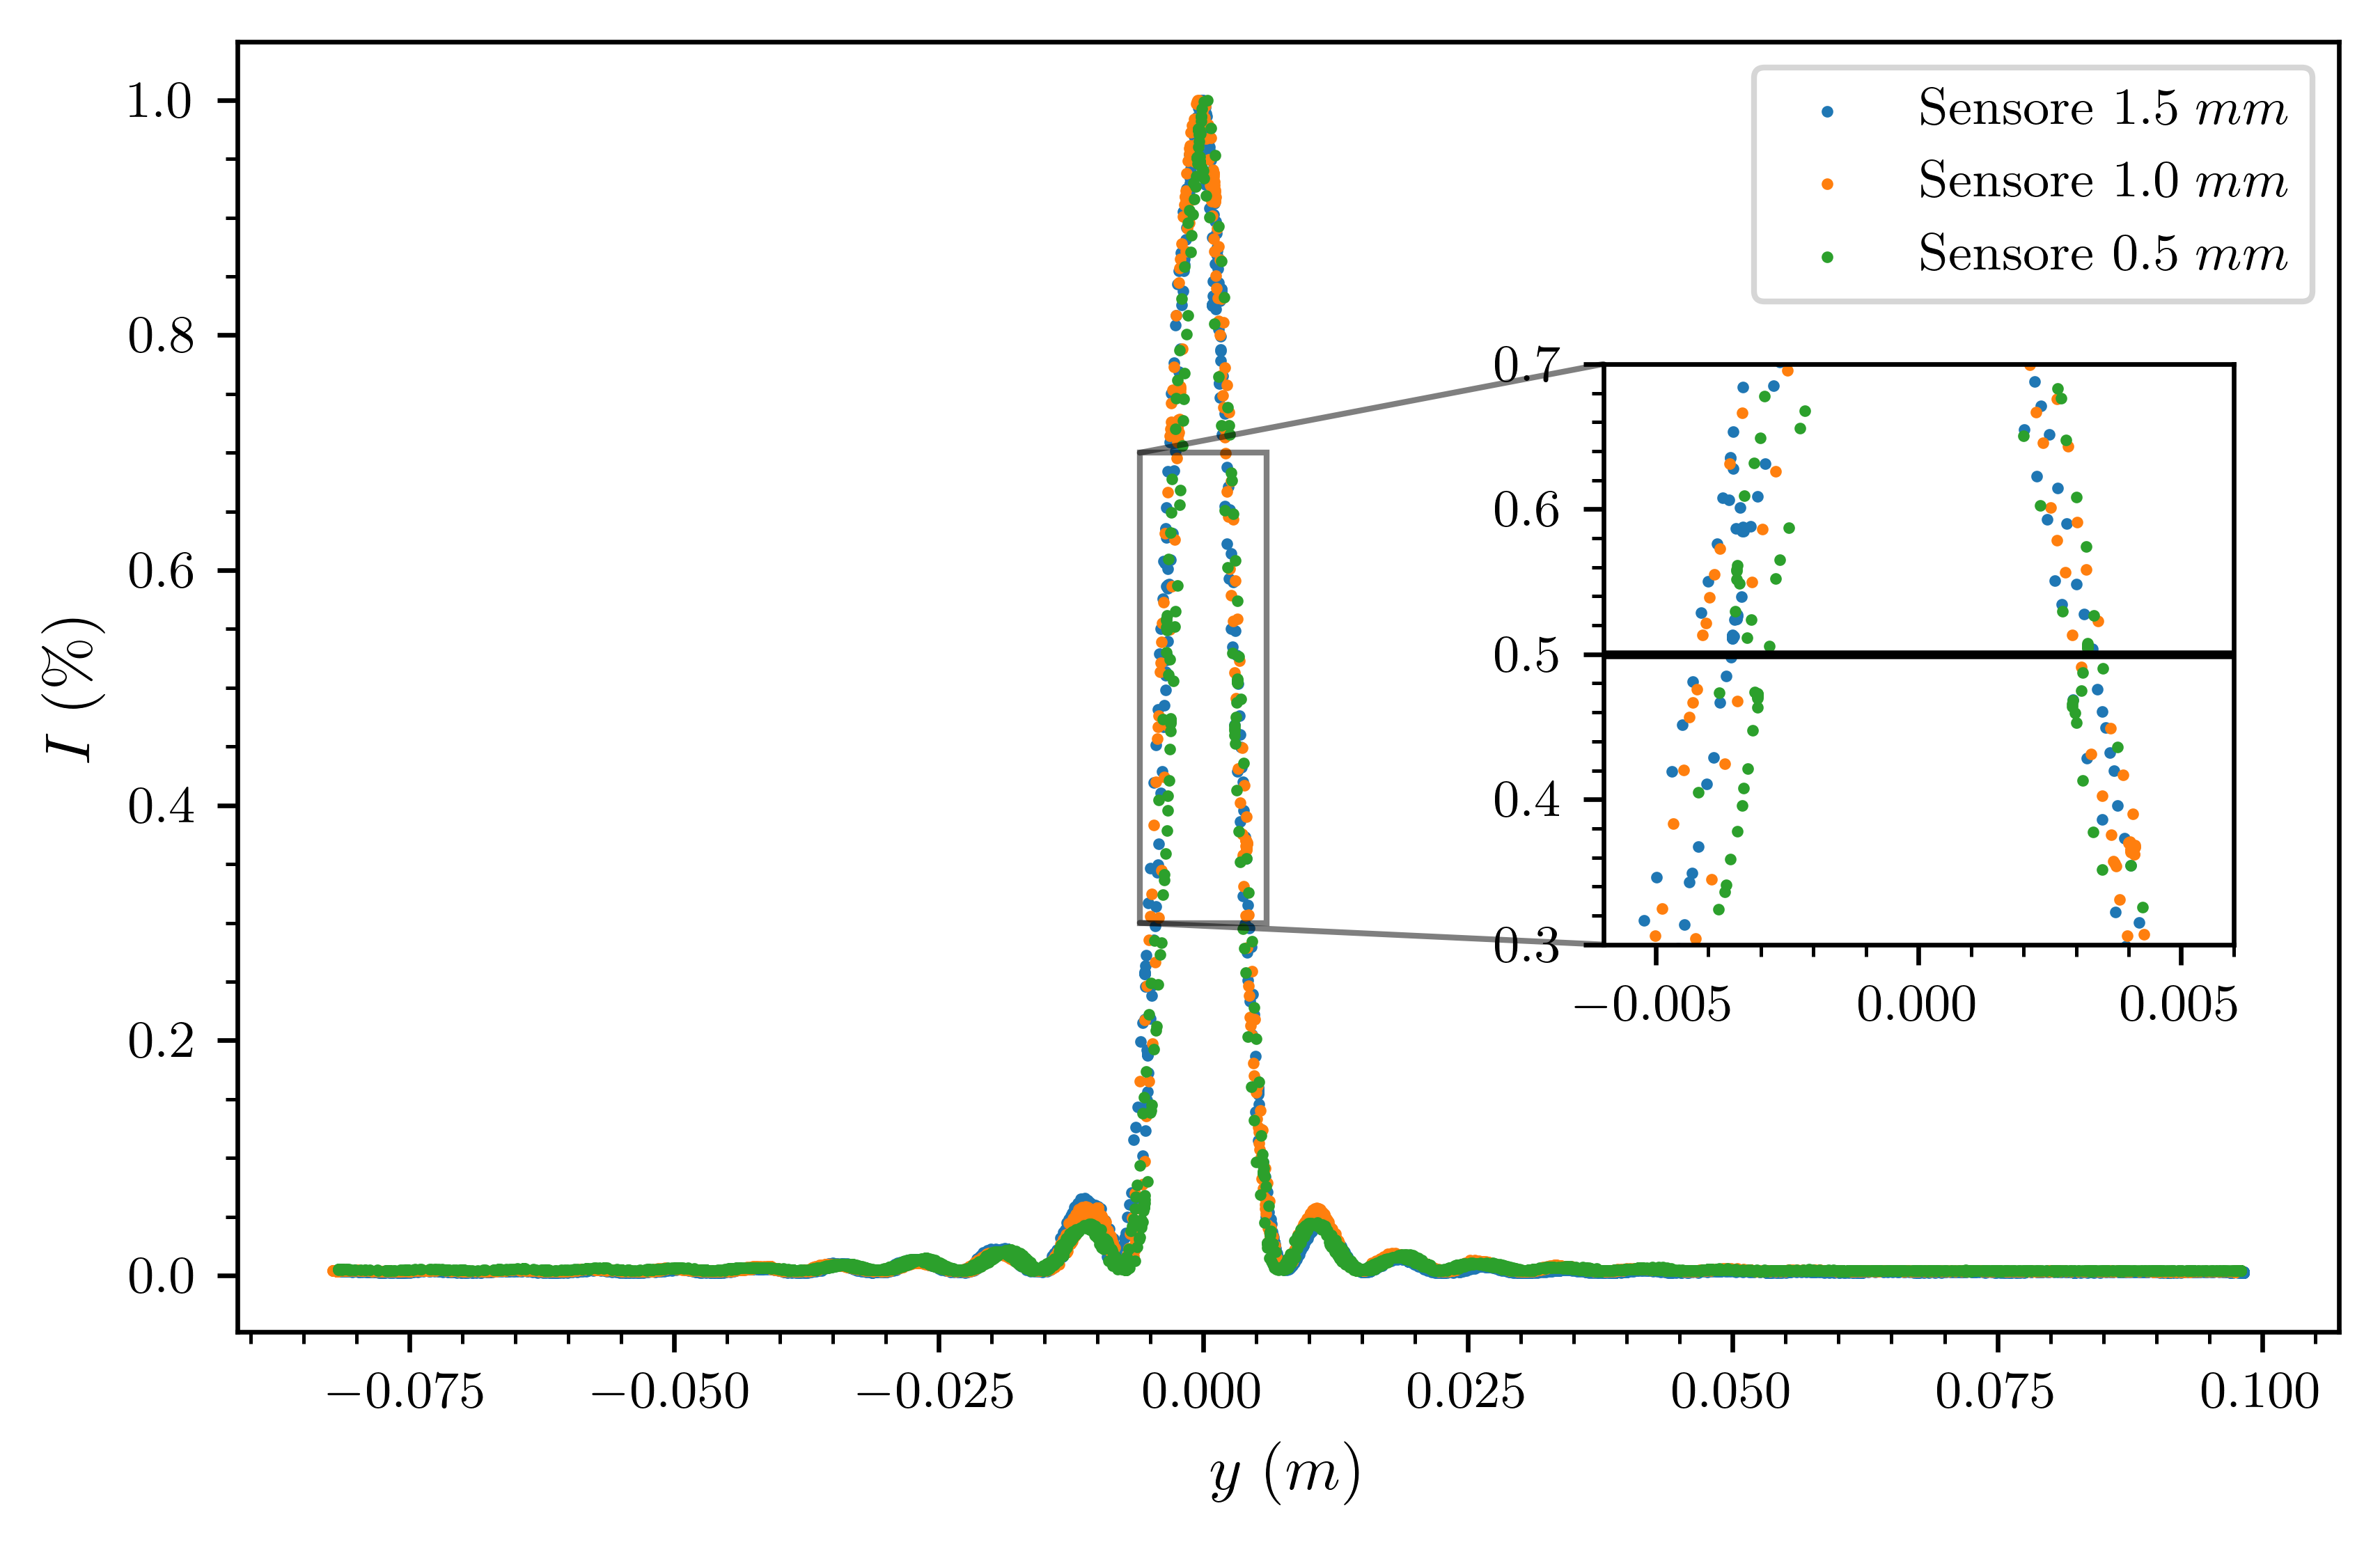
\includegraphics{sensor_0.08.png}
    \caption{Grafico dell'intensità luminosa relativa $I$ in funzione della posizione $y$ (in metri) per ciascuna delle due aperture del sensore.
        Tutti i set sono stati misurati con il fondoscala intermedio (\textit{lampadina}). I valori delle intensità sono stati scalati in modo che l'altezza del picco centrale fosse pari a $1$, questo permette di confrontare i picchi con più semplicità.
        Per quanto il set effettuato con un'apertura pari a \qty{0.5}{\mm} abbia un picco centrale leggermente più stretto rispetto agli altri due, una relazione simile non può essere individuata confrontando i set a \qty{1.5}{\mm} e \qty{1.0}{\mm}. In conclusione non è possibile estrapolare una relazione tra la dimensione dell'apertura e la larghezza del picco centrale.}
    \label{fig:sensore 0.08}
\end{figure}

\end{document}